% Présentation beamer pour un manager : leçons de la simulation S-DBR (mini-usine 10 postes).
% Compilation (depuis le dossier sdbr-mini-usine/) :
%   pdflatex -interaction=nonstopmode rapport-manager.tex  (deux fois)
% Paquets requis : beamer, lmodern, graphicx, booktabs (texlive standard).
\documentclass[10pt,aspectratio=169]{beamer}
\usepackage[utf8]{inputenc}
\usepackage[T1]{fontenc}
\usepackage{lmodern}
\usepackage{graphicx}
\usepackage{booktabs}
\usetheme{Boadilla}
\setbeamertemplate{navigation symbols}{}
\title[Lancer plus tôt ne livre pas plus tôt]{Lancer plus tôt ne livre pas plus tôt}
\subtitle{Ce que la simulation S-DBR de la mini-usine apprend aux managers}
\author{Projet IndEng --- branche \texttt{vibe/sdbr-mini-usine-eddd3f} (PR \#2)}
\date{\today}

\begin{document}

\begin{frame}
\titlepage
\begin{center}
\small
Ligne de 10 postes à goulot central --- Monte-Carlo (10 graines appariées) ---\\
vérification des écrits de Goldratt, \emph{Standing on the Shoulders of Giants} (2006)
\end{center}
\end{frame}

\begin{frame}{Pourquoi cette étude ?}
\begin{itemize}
  \item Objectif managérial : tenir l'\textbf{OTD} (\% d'ordres de fabrication livrés à l'heure).
  \item La tentation est de \textbf{lancer tôt} pour « occuper » l'atelier et rassurer le client.
  \item Goldratt répond : on lance à \emph{échéance $-$ tampon} (la « corde » du DBR) --- lancer plus tôt
        ne fait qu'augmenter l'\textbf{encours} sans augmenter le débit.
  \item Questions testées ici : \textbf{quelle taille de fenêtre de lancement ?} et
        \textbf{quelle politique de lots} (regroupements par famille) ?
  \item Méthode : le Monte-Carlo du simulateur HTML rejoué, plus un moteur Python paramétrable,
        campagnes à \textbf{graines appariées} (les mêmes 10 graines pour toutes les variantes),
        intervalles de confiance à 95\,\%.
\end{itemize}
\end{frame}

\begin{frame}{Ce que prédit Goldratt (2006) --- et ce que la simulation confirme}
\small
\begin{tabular}{@{}p{5.6cm}p{6.2cm}@{}}
\toprule
Affirmation (pages de l'article) & Mesure Monte-Carlo \\
\midrule
En surcharge, l'OTD chute « sous 90\,\% » (p.~9) & OTD = 87,3\,\% à 99\,\% de charge du goulot ; $>$ 99\,\% jusqu'à 85\,\% \\
Le temps opératoire $\approx$ 10\,\% du délai total (p.~11) & touch $\approx$ 8--16\,\% du délai client selon la charge \\
Zones vert/jaune/rouge/noir du tampon (p.~15) & 53\,\% des OF dans le 1\textsuperscript{er} tiers, 87\,\% dans les 2 premiers (tampon 90 h) \\
Règle des 5--10\,\% de rouges pour piloter le tampon (p.~16) & 90 h $\rightarrow$ 12,6\,\% de rouges ; 120 h $\rightarrow$ 4,7\,\% : la bande 5--10\,\% est entre les deux \\
Capacité protectrice hors goulot (p.~10) & À 90\,\% sur le goulot, les autres postes tournent à $\approx$ 37--40\,\% \\
Le débit est fixé par la contrainte, pas par les efficacités locales (p.~3, 16--17) & Débit identique quelle que soit la politique de lancement ; cibler un mauvais poste à 90\,\% fait tomber l'OTD à 0,1\,\% \\
\bottomrule
\end{tabular}
\vspace{2pt}
\footnotesize 14 affirmations vérifiées quantitativement (README \S 4, campagnes \texttt{results/}).
\end{frame}

\begin{frame}{Le modèle simulé}
\begin{itemize}
  \item \textbf{Ligne de 10 postes en série}, goulot central (5--7 h + 2 h de réglage,
        postes réguliers 5,4 h : surcapacité $\times 1{,}25$), tampons interpostes finis (16 OF).
  \item \textbf{Travail total} $W \approx 54{,}3$ h par OF ; 4 familles de produits (mêmes gammes).
  \item \textbf{Demande} : arrivées Poisson (CV 1), délai client demandé lognormal, moyenne 12 $\times W$,
        entre 10 et 40 $\times W$ ; phases de charge 0,70 / 0,95 / 1,30 / 0,85.
  \item \textbf{Lancement} : à \emph{max(arrivée, échéance $-$ fenêtre)}, fenêtre balayée de 1 à 45 $\times W$.
  \item \textbf{Lots} : regroupement par famille à chaque poste, plafond \texttt{size} = 16,
        lot minimum paramétrable avec attente bornée (168 h) ; transfert unitaire.
  \item \textbf{Répétitions} : 10 graines appariées par point, warm-up 400 h,
        900 simulations par campagne.
\end{itemize}
\end{frame}

\begin{frame}{Résultat 1 --- le « U » de l'OTD selon la fenêtre de lancement}
\begin{columns}[T]
\begin{column}{0.55\textwidth}
  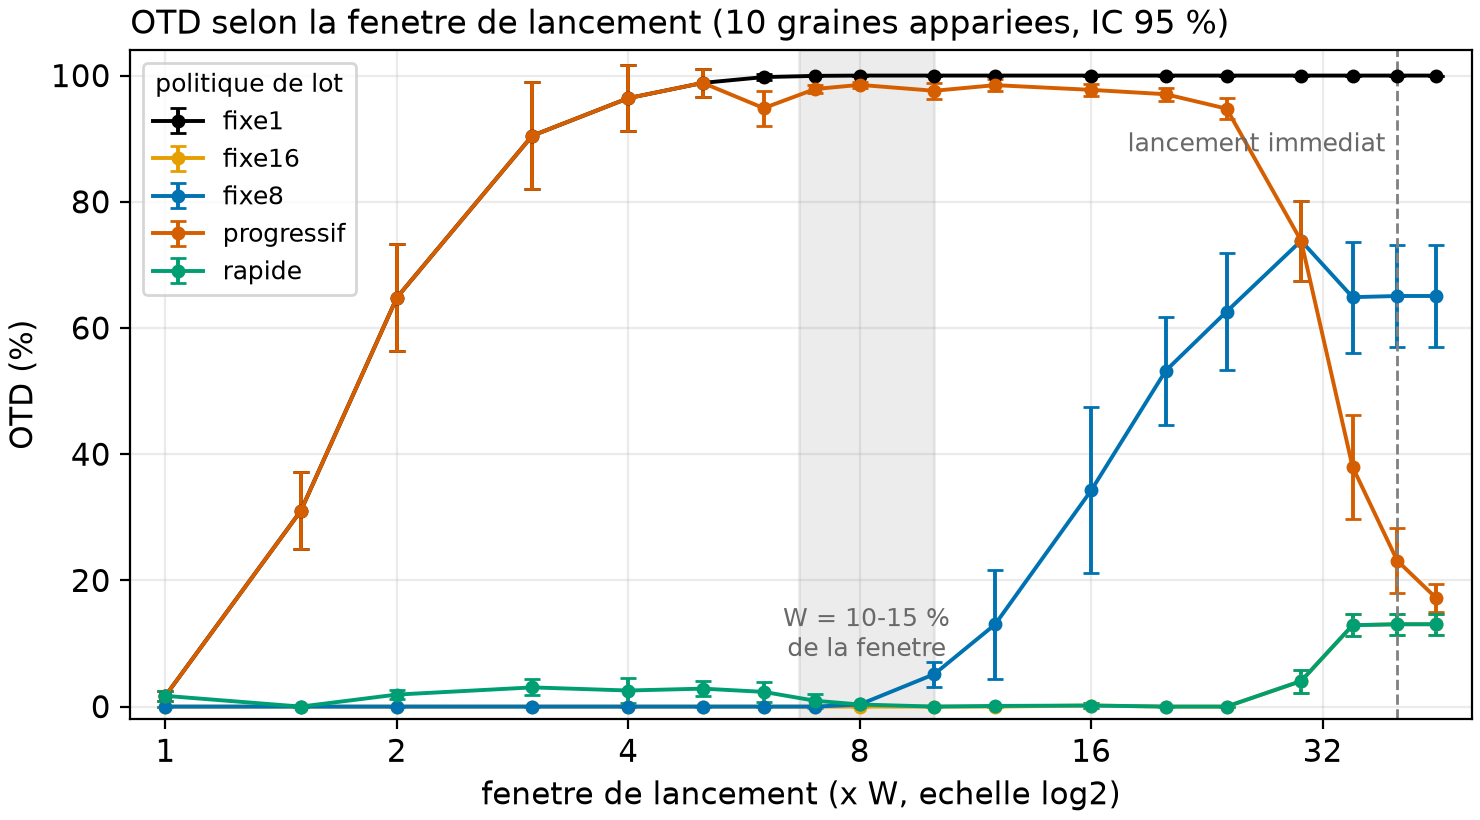
\includegraphics[width=\linewidth]{results/figure-u/slide_otd.png}
\end{column}
\begin{column}{0.42\textwidth}
\small
\begin{itemize}
  \item \textbf{Branche gauche} (fenêtre trop courte) : ruptures de charge, changements de série,
        OTD effondré (1,7\,\% à 1$\times W$).
  \item \textbf{Pic} : 98,5\,\% à 8$\times W$ pour la politique progressive ---
        soit $W \approx 12{,}5$\,\% de la fenêtre, la bande 10--15\,\% de Goldratt.
  \item \textbf{Branche droite} : à 45$\times W$, les regroupements dominent :
        17,2\,\% seulement (politique progressive).
  \item Sans lot minimum (fixe1, noir), l'OTD reste à 100\,\% : la branche droite
        vient des \textbf{lots}, pas de la fenêtre seule.
\end{itemize}
\end{column}
\end{columns}
\end{frame}

\begin{frame}{Résultat 2 --- dans quel tiers de la fenêtre les OF se terminent-ils ?}
\begin{columns}[T]
\begin{column}{0.55\textwidth}
  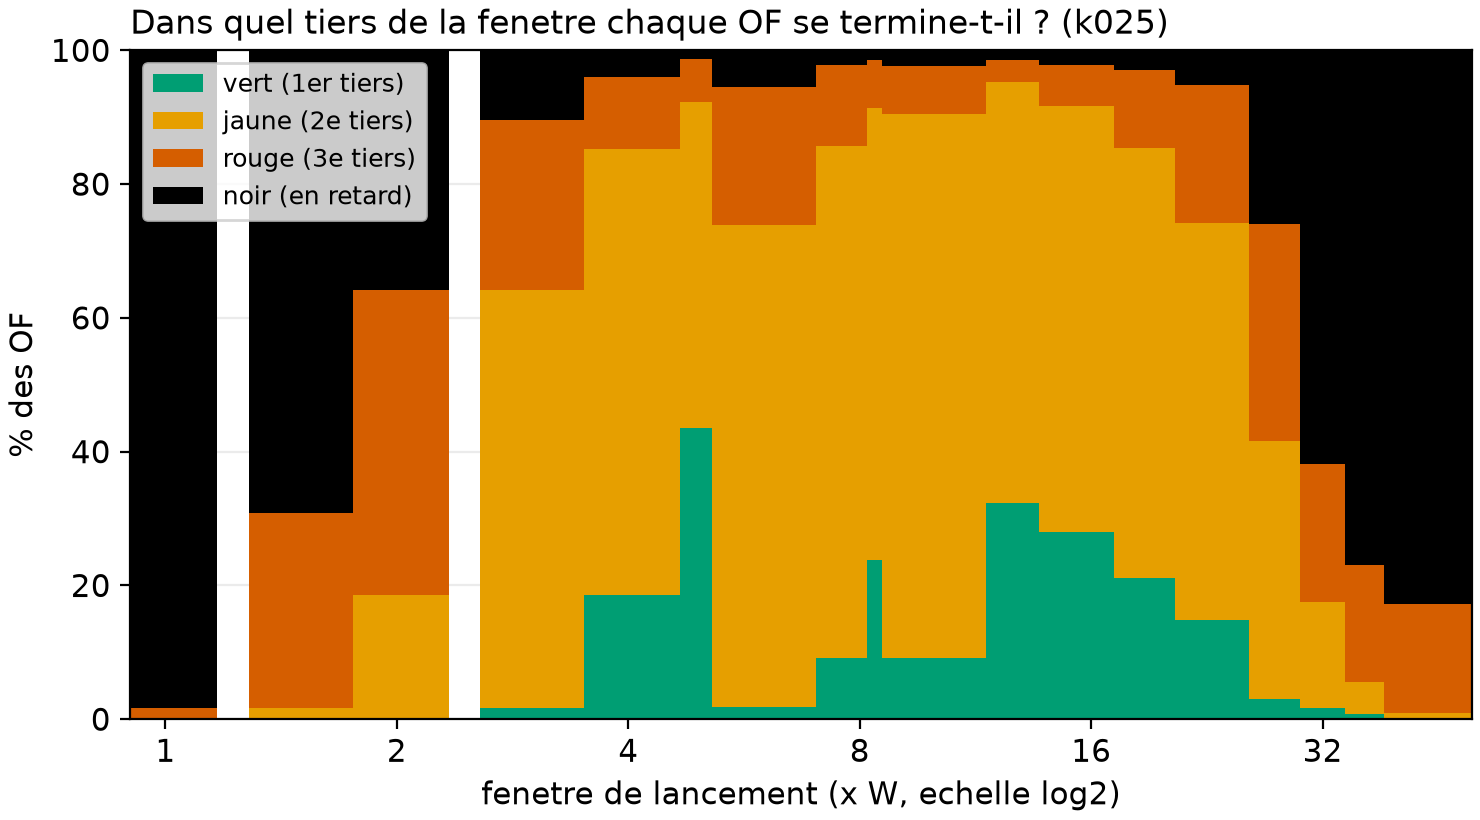
\includegraphics[width=\linewidth]{results/lot-fenetre-coef/slide_zones.png}
\end{column}
\begin{column}{0.42\textwidth}
\small
\begin{itemize}
  \item Zones de Goldratt (p.~15) : vert = 1\textsuperscript{er} tiers de la fenêtre, jaune = 2\textsuperscript{e},
        rouge = 3\textsuperscript{e}, noir = en retard.
  \item Fenêtre 5--8$\times W$ : $\approx$ 90\,\% des OF en vert/jaune, 1,5--4\,\% en retard.
  \item Fenêtre 45$\times W$ : \textbf{83\,\% d'OF noirs} (fin à 1,7$\times$ la fenêtre après lancement).
  \item Leçon : piloter au \textbf{nombre de rouges/noirs} (règle des 5--10\,\%, p.~16),
        pas au réordonnancement fin à l'intérieur d'une même zone (p.~14--15).
\end{itemize}
\end{column}
\end{columns}
\end{frame}

\begin{frame}{Résultat 3 --- le mécanisme : lots réalisés et encours}
\begin{columns}[T]
\begin{column}{0.55\textwidth}
  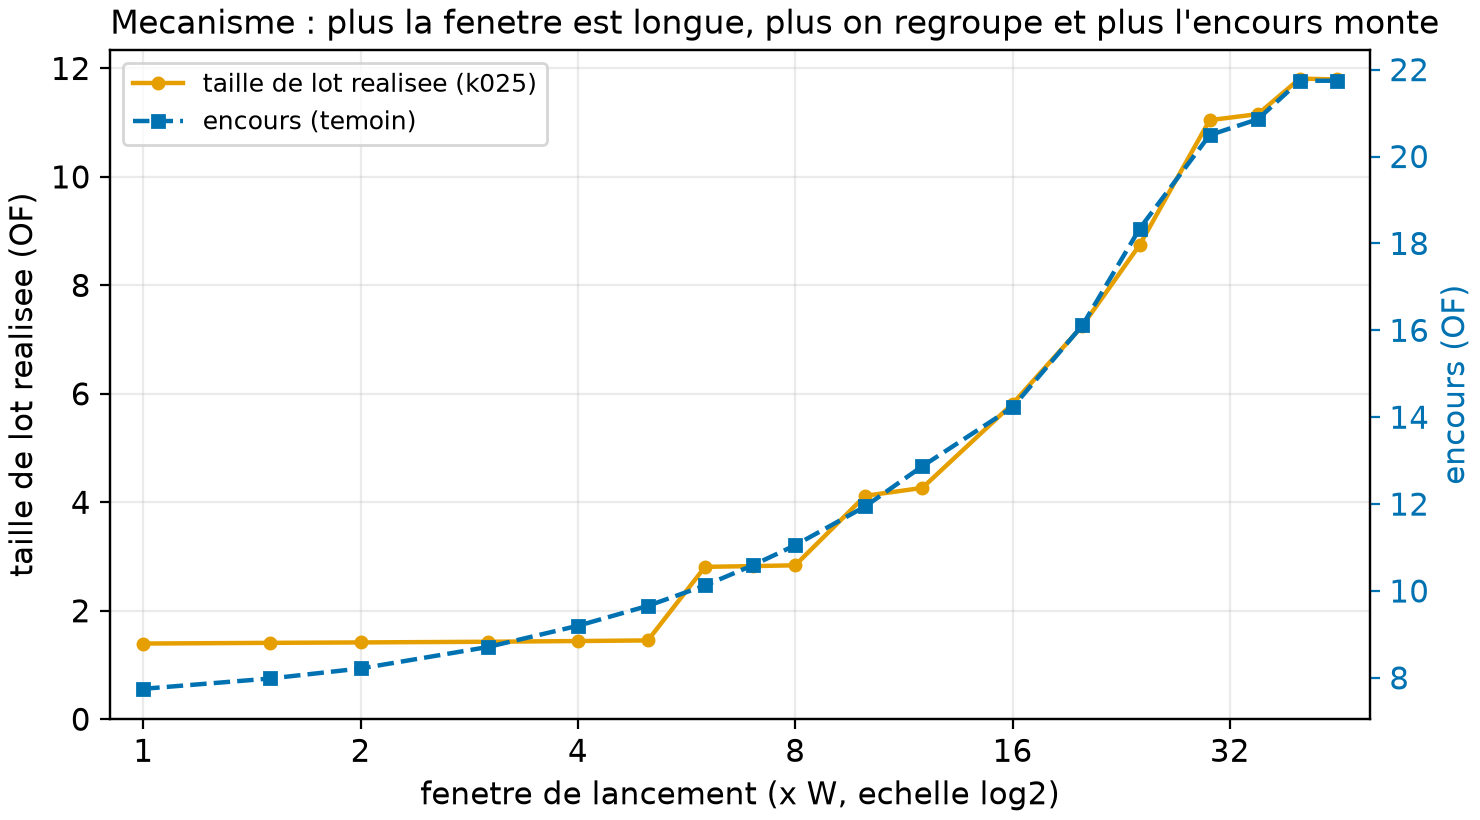
\includegraphics[width=\linewidth]{results/lot-fenetre-coef/slide_meca.png}
\end{column}
\begin{column}{0.42\textwidth}
\small
\begin{itemize}
  \item Plus la fenêtre est longue, plus le lot pratiqué grossit (1,4 $\rightarrow$ 11,8 OF).
  \item Et plus l'encours explose : 22 $\rightarrow$ 175 OF ($\times 8$), loi de Little vérifiée
        (encours = débit $\times$ traversée).
  \item Au goulot, l'attente pour \textbf{remplir le lot minimum} atteint 220--870 h
        ($\approx$ 4--16$\times W$) ; les conflits (OF urgents dépassés par un lot) passent
        de $\approx$ 0 à 160--200.
\end{itemize}
\end{column}
\end{columns}
\end{frame}

\begin{frame}{Résultat 4 --- imposer un lot minimum fixe (2 / 4 / 8 / 16)}
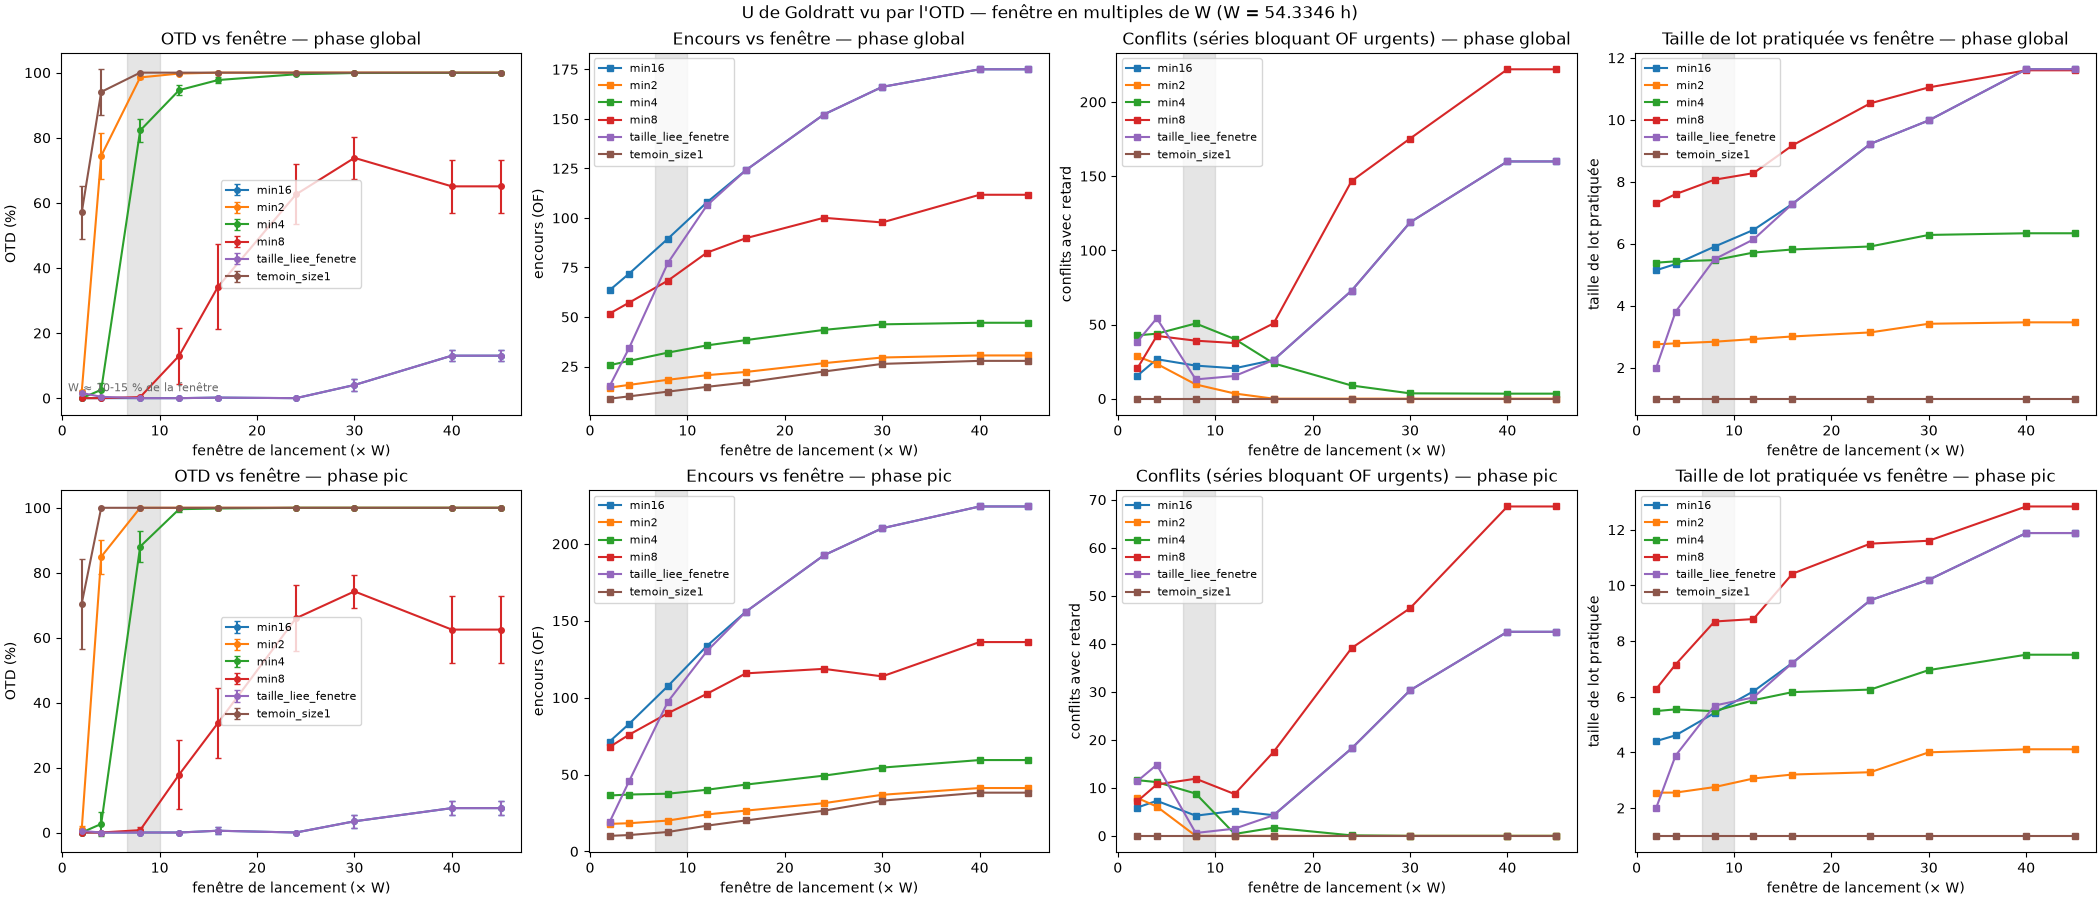
\includegraphics[width=0.92\linewidth]{results/lot-min-40xw/u_otd.png}
\vspace{4pt}
\small
\begin{itemize}
  \item Avec une attente de remplissage de 168 h, les lots se forment vraiment (taille pratiquée 11,6/16)
        et l'OTD s'effondre à grande fenêtre : \textbf{min16 $\rightarrow$ 13\,\% à 40--45$\times W$},
        min8 trace un U (0\,\% $\rightarrow$ 74\,\% à 30$\times W$ $\rightarrow$ 65\,\%).
  \item Leçon : \textbf{ne pas attendre pour former de gros lots au goulot} --- chaque heure
        d'attente pour remplir un lot est une heure de retard pour tout le lot.
\end{itemize}
\end{frame}

\begin{frame}{Résultat 5 --- dimensionner le lot minimum par la fenêtre : lot min $= k \times$ fenêtre $/W$}
\begin{columns}[T]
\begin{column}{0.52\textwidth}
  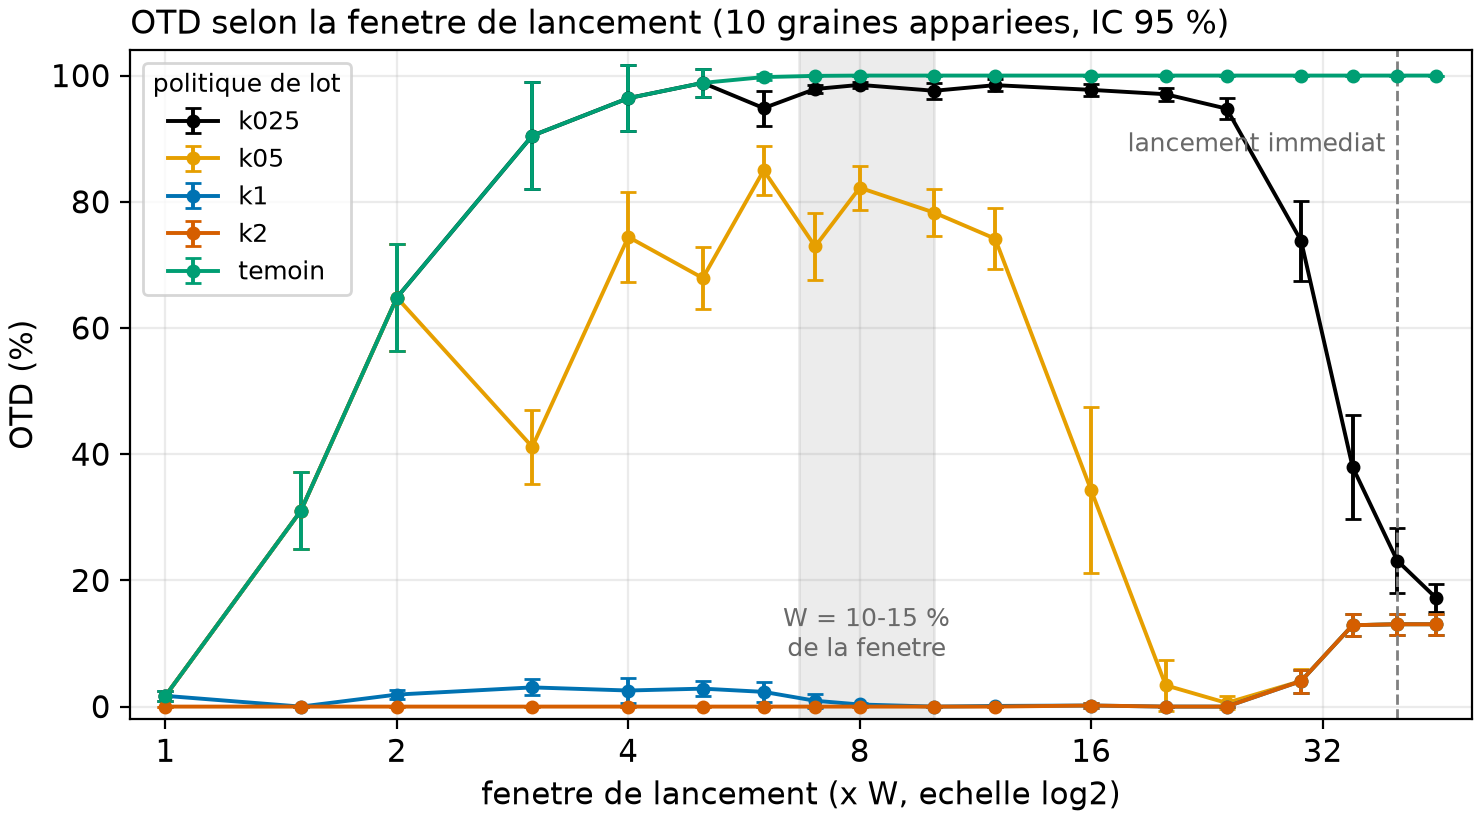
\includegraphics[width=\linewidth]{results/lot-fenetre-coef/slide_otd.png}
\end{column}
\begin{column}{0.45\textwidth}
\small
OTD (\%) à quelques fenêtres :
\begin{tabular}{@{}lcccc@{}}
\toprule
$\times W$ & 2 & 8 & 16 & 45 \\
\midrule
témoin (min 1) & 64,8 & 100 & 100 & 100 \\
k = 0,25 & 64,8 & \textbf{98,5} & 97,7 & 17,2 \\
k = 0,5  & 64,8 & 82,2 & 34,3 & 13,1 \\
k = 1 (fenêtre/W) & 1,9 & 0,3 & 0,2 & 13,1 \\
k = 2    & 0,0 & 0,0 & 0,2 & 13,1 \\
\bottomrule
\end{tabular}
\vspace{3pt}
\begin{itemize}
  \item Seul \textbf{$k = 0{,}25$} (lot min = fenêtre$/4W$) trace le U complet (pic 98,8\,\% à 5$\times W$).
  \item La règle « lot min = fenêtre$/W$ » ($k=1$) est $\approx$ 4$\times$ trop agressive : OTD $\approx$ 0 dès 2$\times W$.
  \item À la fenêtre optimale, le lot minimum supportable est \textbf{$\leq 2$ OF}.
\end{itemize}
\end{column}
\end{columns}
\end{frame}

\begin{frame}{Résultat 6 --- comparaison appariée : lots fixes vs lot lié à la fenêtre}
\begin{columns}[T]
\begin{column}{0.55\textwidth}
  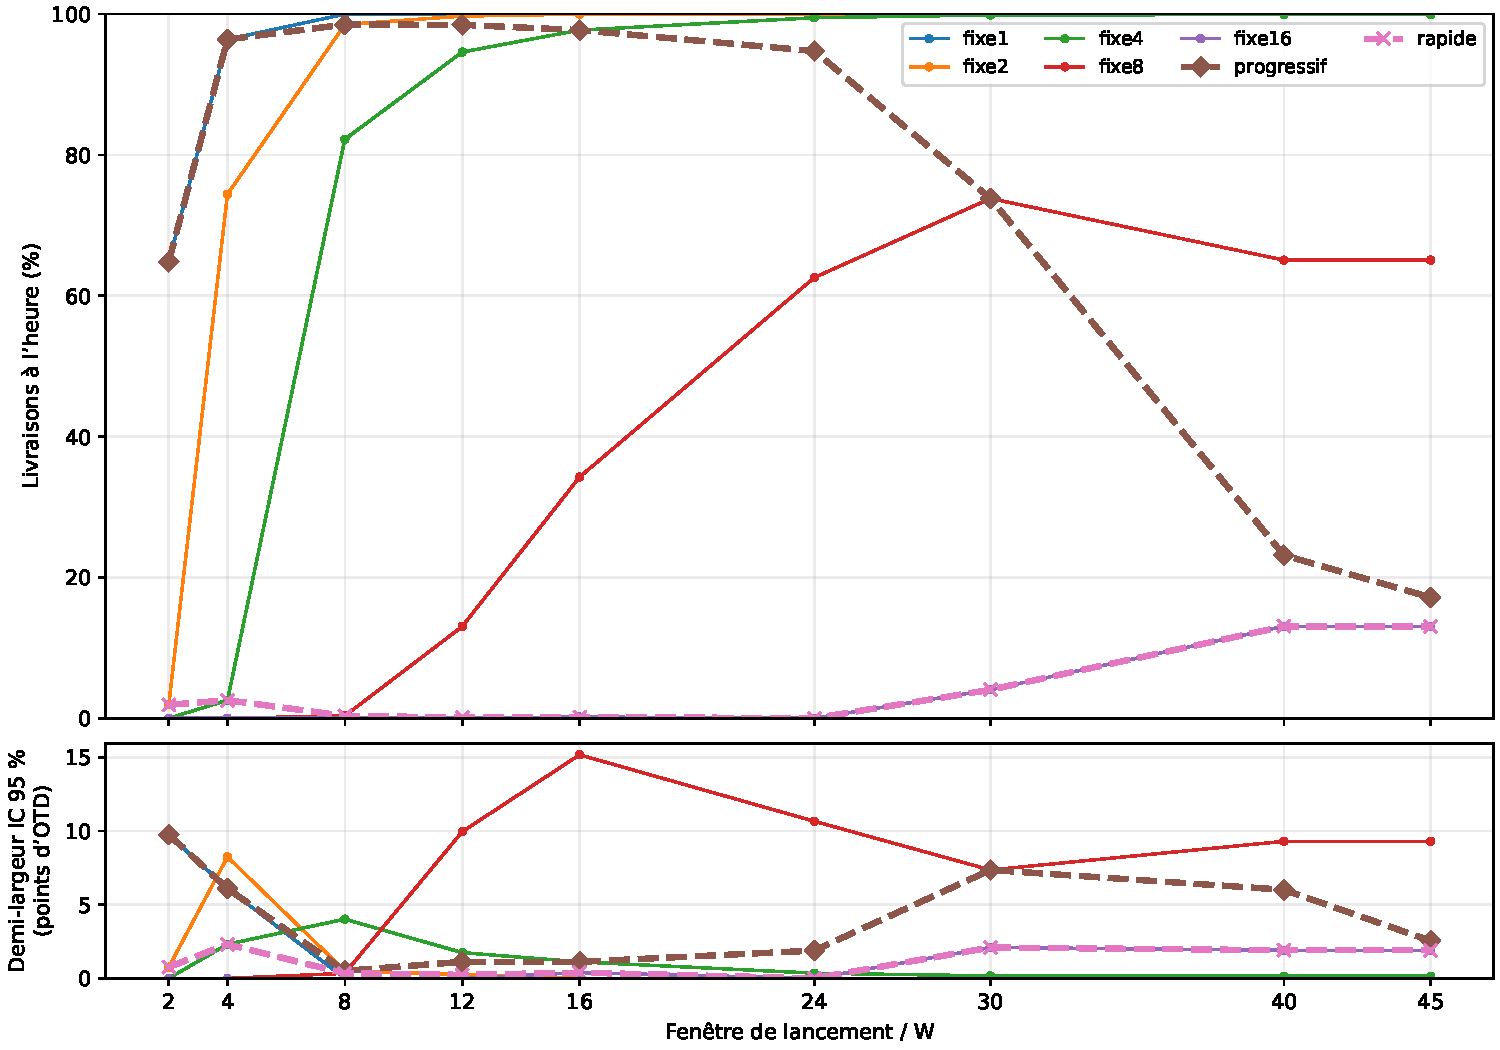
\includegraphics[width=\linewidth]{results/iso-lot/otd-fenetre.pdf}
\end{column}
\begin{column}{0.42\textwidth}
\small
\begin{itemize}
  \item Même ligne, mêmes graines (42--51) pour chaque politique.
  \item \textbf{Lot min 1 + fenêtre 8$\times W$} : OTD 100\,\% de 8 à 45$\times W$ --- l'optimum.
  \item Lot min progressif ($k=0{,}25$) : 98,5\,\% à 8$\times W$ mais \textbf{17,2\,\% à 45$\times W$};
        écart apparié à 45$\times W$ : \textbf{+82,8 points} [IC 80,3 ; 85,4] pour le lot min 1.
  \item Au-delà de 40$\times W$ = lead max : lancement immédiat, toutes les variantes au même niveau
        de base (13\,\% quand le lot min atteint le plafond 16).
\end{itemize}
\end{column}
\end{columns}
\end{frame}

\begin{frame}{Résultat 7 --- la surcharge tue l'OTD, quoi que l'on fasse}
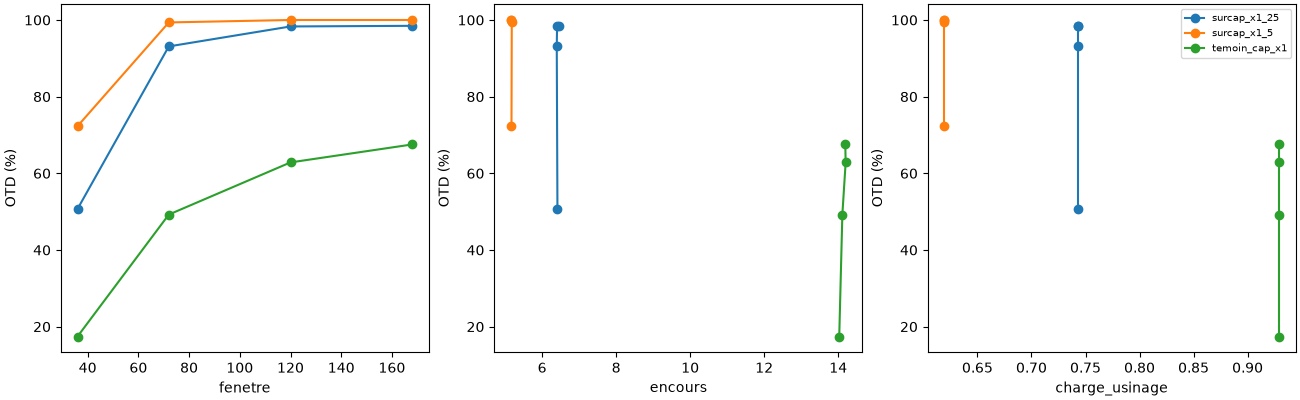
\includegraphics[width=0.72\linewidth]{results/surcharge-10-postes/otd.png}
\vspace{2pt}

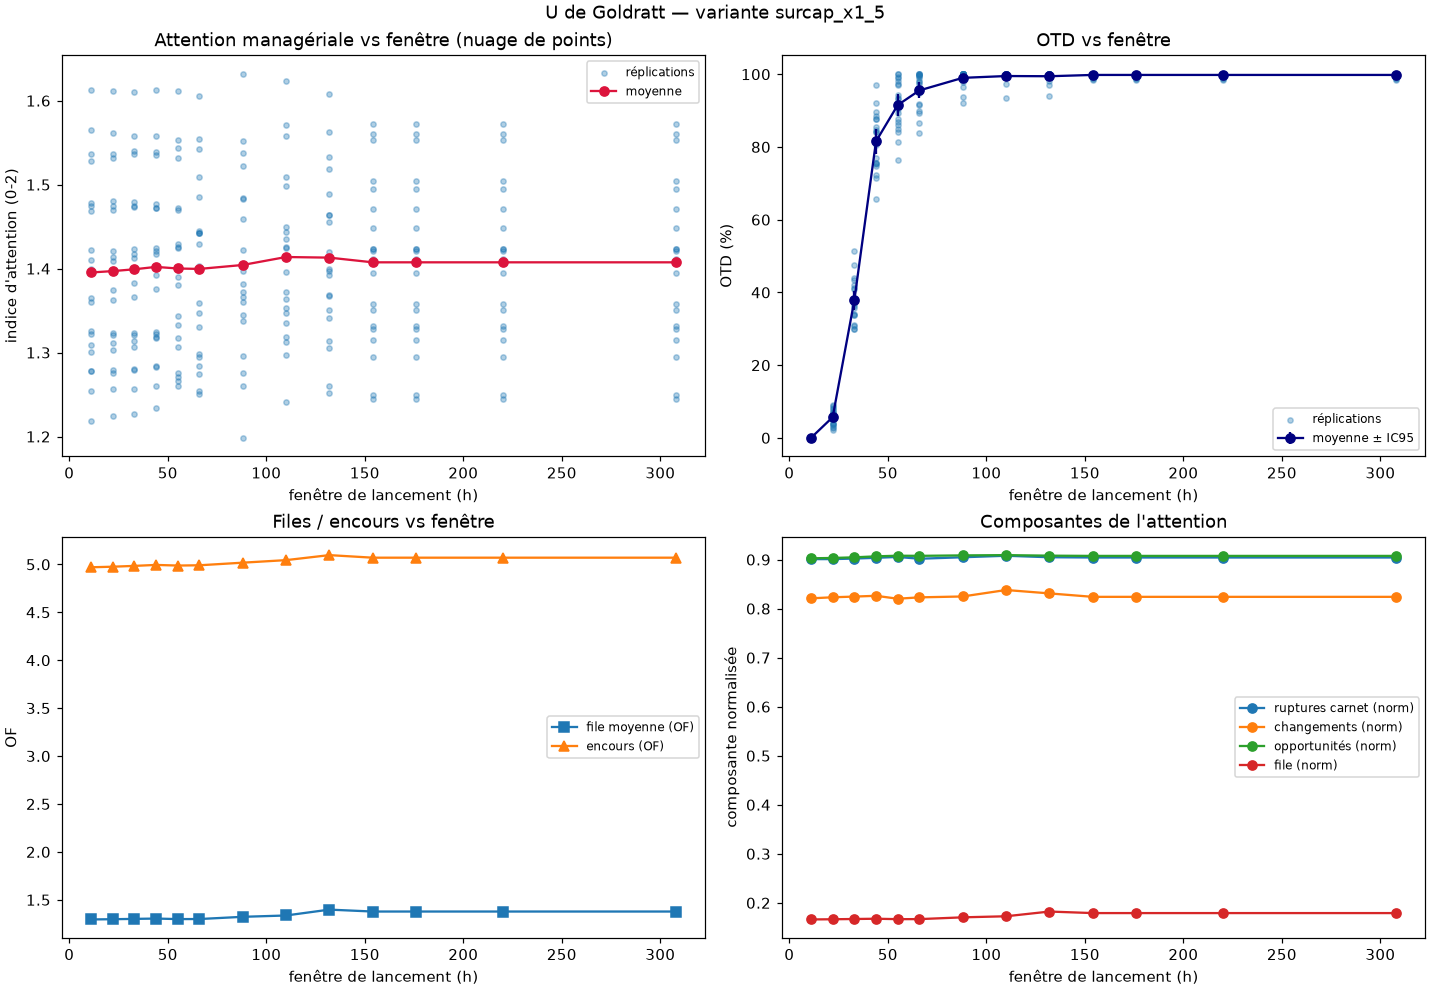
\includegraphics[height=0.42\textheight]{results/dashboard-u/u_surcap_x1_5.png}
\vspace{2pt}
\small
\begin{itemize}
  \item Quand la charge offerte approche 100\,\% du goulot ($\rho \rightarrow 1$), l'OTD passe de
        96\,\% à 33\,\% et l'encours est $\times 5$ : effet non linéaire des fluctuations (p.~14, « jeu de dés »).
  \item Leçon : en surcharge, \textbf{gérer la charge en amont} (carnet, délais client), pas la fenêtre.
\end{itemize}
\end{frame}

\begin{frame}{Leçons pour un manager}
\begin{enumerate}
  \item \textbf{Ne lancez pas plus tôt que la fenêtre utile} : la corde (fenêtre = échéance $-$ tampon)
        borne l'encours ; au-delà, on achète du retard, pas du débit (loi de Little vérifiée).
  \item \textbf{Dimensionnez la fenêtre pour que $W \approx 10$--$15\,\%$ de la fenêtre}
        (ici pic à 5--8$\times W$, OTD $\approx$ 98--100\,\%).
  \item \textbf{Pilotez au tampon par les zones vert/jaune/rouge/noir} et à la règle des 5--10\,\% de rouges ;
        le réordonnancement fin à l'intérieur d'une zone n'apporte presque rien.
  \item \textbf{Pas de grand lot minimum imposé} : attendre pour remplir un lot bloque le goulot
        (220--870 h d'attente mesurées) ; à la fenêtre optimale, lot min $\leq 2$.
        Règle testée : lot min $\approx$ fenêtre$/(4W)$, pas fenêtre$/W$.
  \item \textbf{Protégez la capacité hors goulot} ($\approx$ 25\,\% de surcapacité) :
        le débit est fixé par le goulot, pas par l'occupation des autres postes.
  \item \textbf{En surcharge ($\rho \to 1$), l'OTD s'effondre} (96 $\rightarrow$ 33\,\%) quel que soit le réglage :
        agir sur la charge, pas sur la fenêtre.
\end{enumerate}
\end{frame}

\begin{frame}{Pistes d'amélioration et limites du modèle}
\small
\begin{itemize}
  \item \textbf{Attention managériale non modélisée} (Fig.~1, p.~12--13) : ajouter pannes, expediting et
        saturation d'attention --- un fort encours masque les vrais problèmes (« rochers et eau », p.~6).
  \item \textbf{Boucle vicieuse dynamique} (p.~14) : retard $\rightarrow$ « on lance plus tôt »
        $\rightarrow$ plus d'encours $\rightarrow$ plus de retard.
  \item \textbf{Promesses pilotées par le client} : avec \emph{lancement = max(arrivée, échéance $-$ fenêtre)},
        l'OTD vs fenêtre est monotone jusqu'à la saturation (fenêtre $\geq$ lead max) ; la branche droite
        apparaît alors comme un \emph{écart de niveau} entre politiques de lots, pas comme une pente.
        Une pente « en chute » suppose des promesses pilotées par la capacité du goulot.
  \item \textbf{DBR ou CCPM ?} : le DBR suppose touch $<$ 10\,\% du délai promis (p.~18) ;
        au-delà (10--30\,\%), passer en CCPM.
  \item \textbf{Moteur déjà en place} : lots à tous les postes, trains logistiques (\texttt{transfer} = N),
        lot minimum avec attente bornée, familles, surcapacité relative, tableaux de bord
        (ruptures, changements de série, opportunités de regroupement).
\end{itemize}
\end{frame}

\begin{frame}{Reproduction et références}
\footnotesize
\begin{itemize}
  \item Tests : \texttt{.venv/bin/python -m pytest -q} (57 tests).
  \item Campagnes : \texttt{sdbr-mini-usine/scenario-*.json} $\rightarrow$
        \texttt{.venv/bin/python sdbr-mini-usine/scripts/run\_hypotheses.py <scénario> --out <dir>}.
  \item Figures : \texttt{scripts/figure\_u.py}, \texttt{scripts/figure\_slides.py},
        \texttt{scripts/zones\_couleur.py}, \texttt{scripts/courbe\_u.py}, \texttt{scripts/dashboard\_u.py}.
  \item Résultats et analyses : \texttt{sdbr-mini-usine/results/*/} et les fichiers
        \texttt{sdbr-mini-usine/*.md} (README \S 1--23, \texttt{pistes-extension.md},
        \texttt{figure-u.md}, \texttt{lot-fenetre-coef.md}, \texttt{lot-min-40xw.md}...).
  \item Cette présentation : \texttt{cd sdbr-mini-usine \&\& pdflatex -interaction=nonstopmode rapport-manager.tex}.
  \item Référence : E.~M.~Goldratt, \emph{Standing on the Shoulders of Giants}, 2006
        (pages citées : 3, 6, 8--18) --- fichier \texttt{goldratt-standing-on-the-shoulders-of-giants.pdf}.
  \item Livraison : branche \texttt{vibe/sdbr-mini-usine-eddd3f}, PR \#2.
\end{itemize}
\end{frame}

\end{document}
